
\documentclass[12pt]{article}
\usepackage[utf8]{inputenc}
\usepackage[spanish]{babel}
\usepackage{amsmath}
\usepackage{geometry}
\usepackage{graphicx}
\usepackage{listings}
\usepackage{color}
\geometry{margin=2.5cm}

\usepackage{listings}
\usepackage{xcolor}

\lstset{
  language=C++,
  basicstyle=\ttfamily\small,
  frame=single,
  breaklines=true,
  postbreak=\mbox{\textcolor{red}{$\hookrightarrow$}\space},
  columns=flexible
}


\title{Paralelización en CUDA: Transformada de Fourier Discreta y Continua}
\author{Jesús Losada Arauzo}
\date{\today}

\begin{document}

\maketitle

\section*{Resumen}

En este informe se analiza la paralelización mediante CUDA de la Transformada de Fourier Discreta (DFT) y versiones continuas con integración numérica. El objetivo es medir el rendimiento frente a la versión secuencial utilizando diferentes técnicas de integración: suma de rectángulos, trapecios y método de Simpson. Se emplea memoria unificada y eventos CUDA para una gestión sencilla de datos y tiempos.

\section*{Paralelización en CUDA}

El programa implementa varios \textit{kernels} CUDA, uno para cada versión de la transformada:

\begin{itemize}
    \item \textbf{DFT}: versión discreta clásica.
    \item \textbf{CFT}: versión continua básica, usando suma directa.
    \item \textbf{CFT\_Trapecio} y \textbf{CFT\_Simpson}: integración continua por métodos numéricos.
\end{itemize}

Se utiliza una distribución fija de hilos: \texttt{BLOCK\_SIZE = 256} y \texttt{NUM\_BLOCKS = 10}. Cada hilo se encarga de calcular una componente del vector de Fourier (una frecuencia). Internamente, el hilo hace un bucle que suma o integra la función con el método correspondiente.

\subsection*{Distribución del trabajo}

Cada hilo CUDA calcula un índice global:

\[
\texttt{i = blockIdx.x * blockDim.x + threadIdx.x}
\]

Con ese índice se decide si se procesa la componente \( i \) del vector de salida. De este modo, la carga de trabajo se distribuye automáticamente entre los hilos, permitiendo ejecutar en paralelo todos los valores de la transformada.

\subsection*{Medición de tiempo}

El tiempo se mide mediante \texttt{cudaEventRecord}, lo cual permite medir con precisión únicamente la ejecución del kernel (sin contar asignaciones ni E/S). El resultado se almacena en archivos para su posterior graficado.

\section*{Resultados obtenidos}

Las siguientes gráficas muestran los tiempos medidos en milisegundos para distintos tamaños de muestra. Se comparan versiones secuenciales y paralelas.

\begin{itemize}
    \item Para muestras pequeñas, CUDA tiene cierta penalización inicial.
    \item A partir de cierto tamaño, la versión paralela supera ampliamente a la secuencial.
\end{itemize}

\begin{figure}[h]
    \centering
    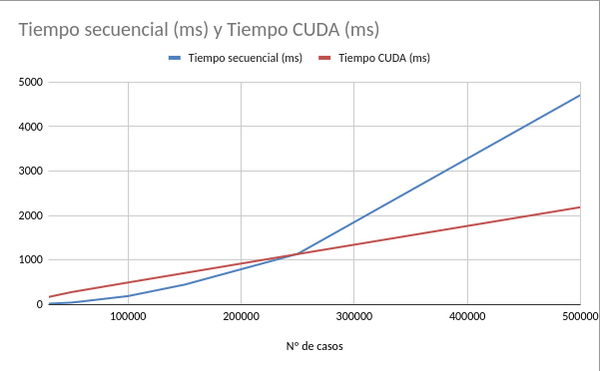
\includegraphics[width=0.8\textwidth]{captura1.png}
    \caption{Tiempo de ejecución - DFT (Transformada Discreta)}
\end{figure}

\begin{figure}[h]
    \centering
    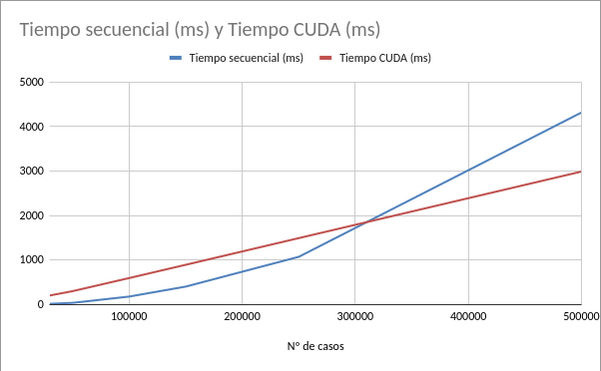
\includegraphics[width=0.8\textwidth]{captura2.png}
    \caption{Tiempo de ejecución - Suma de Rectángulos}
\end{figure}

\begin{figure}[h]
    \centering
    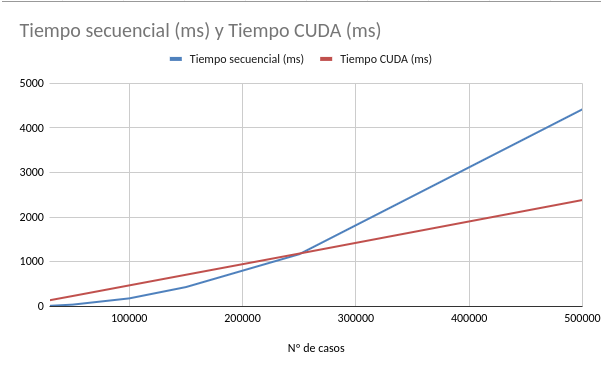
\includegraphics[width=0.8\textwidth]{captura3.png}
    \caption{Tiempo de ejecución - Método del Trapecio}
\end{figure}

\begin{figure}[h]
    \centering
    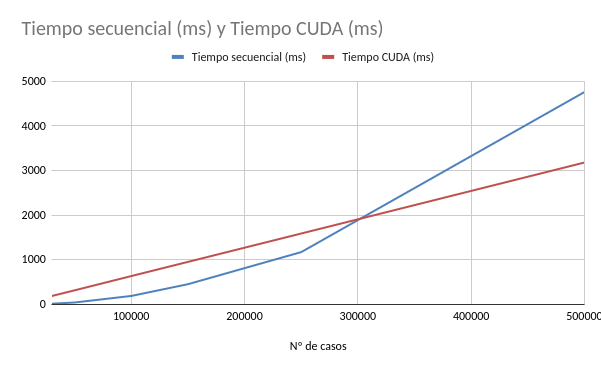
\includegraphics[width=0.75\linewidth]{captura4.png}
    \caption{Tiempo de ejecución - Método de Simpson}
\end{figure}

\newpage

\section*{Código CUDA resumido}

\begin{lstlisting}[language=C++, basicstyle=\ttfamily\small, frame=single]
__global__ void DFT(cuDoubleComplex *Fourier, const double *muestras, int N){
    int i = blockIdx.x * blockDim.x + threadIdx.x;
    if (i < N){
        cuDoubleComplex sum = make_cuDoubleComplex(0.0, 0.0);
        for (int j = 0; j < N; j++){
            double angle = -2.0 * PI * i * j / N;
            cuDoubleComplex term = make_cuDoubleComplex(muestras[j]*cos(angle),
                                                        muestras[j]*sin(angle));
            sum = cuCadd(sum, term);
        }
        Fourier[i] = sum;
    }
}

__global__ void CFT(cuDoubleComplex *Fourier, const double *muestras, const int TAM_VECTOR_MUESTRAS, const double paso_temporal){
    int i = blockIdx.x * blockDim.x + threadIdx.x;
    if (i < TAM_VECTOR_MUESTRAS){
        Fourier[i] = make_cuDoubleComplex(0.0,0.0);
        cuDoubleComplex sum = make_cuDoubleComplex(0.0,0.0);
        double omega = 2.0*PI*i/(T_MAX-T_MIN);//La w de la formula que es el omega
        //Aqui ya entra en juego tanto el intervalo del tiempo como los valores que dan la funcion, es decir el tiempo esta entre -1 y 1
        //y los valores de la funcion están en mis muestras
        //Vamos desde el minimo hasta el maximo pero con nuestro paso temporal para tomar fourier lo más preciso posible
        for (double j = T_MIN;j<T_MAX; j= j+paso_temporal){
            //printf("Estoy en el segundo FOR");
            int indice = (int)((j - T_MIN)/paso_temporal);
            if (indice <= 0 ){
                // Si es menor o igual a 0, suponemos que coge el primer elemento
                cuDoubleComplex expo = cuCexp(make_cuDoubleComplex(0.0, -omega * j));  
                cuDoubleComplex temp = make_cuDoubleComplex(muestras[0], 0.0);  
                cuDoubleComplex prod = cuCmul(temp, expo);  
                sum = cuCadd(sum, cuCmulReal(prod, paso_temporal));  
            }
            else if (indice >= TAM_VECTOR_MUESTRAS - 1) { 
                // Si es mayor o igual al número de elementos, cogemos el último
                cuDoubleComplex expo = cuCexp(make_cuDoubleComplex(0.0, -omega * j));  
                cuDoubleComplex temp = make_cuDoubleComplex(muestras[TAM_VECTOR_MUESTRAS - 1], 0.0);  
                cuDoubleComplex prod = cuCmul(temp, expo);  
                sum = cuCadd(sum, cuCmulReal(prod, paso_temporal));  
            } else {
                // Si no es válido y cogemos el valor calculado
                cuDoubleComplex expo = cuCexp(make_cuDoubleComplex(0.0, -omega * j));  // Usamos la función cuCexp para la exponencial
                cuDoubleComplex temp = make_cuDoubleComplex(muestras[indice], 0.0);  // Tomamos la muestra correspondiente
                cuDoubleComplex prod = cuCmul(temp, expo);  // Multiplicamos la muestra por la exponencial
                sum = cuCadd(sum, cuCmulReal(prod, paso_temporal));  // Acumulamos el resultado, aplicando el paso temporal
            }
        }
        Fourier[i] = sum;
    }    
}

__global__ void CFT_Simpson(cuDoubleComplex *Fourier, const double *muestras, const int TAM_VECTOR_MUESTRAS, const double paso_temporal){

        int i = blockIdx.x * blockDim.x + threadIdx.x;
        if (i < TAM_VECTOR_MUESTRAS){
            Fourier[i] = make_cuDoubleComplex(0.0,0.0);
            cuDoubleComplex sum = make_cuDoubleComplex(0.0,0.0);
            double omega = 2.0*PI*i/(T_MAX-T_MIN);//La w de la formula que es el omega

            for (double j = T_MIN;j<T_MAX - paso_temporal; j += paso_temporal){
                int indice1 = (int)((j - T_MIN)/paso_temporal);
                int indice2 = indice1 + 1;

                if (indice2 >= TAM_VECTOR_MUESTRAS) indice2 = TAM_VECTOR_MUESTRAS - 1;
                
                double x_medio = j + paso_temporal / 2.0;
                int indice_medio = (int)((x_medio - T_MIN) / paso_temporal);

                if (indice_medio >= TAM_VECTOR_MUESTRAS) indice_medio = TAM_VECTOR_MUESTRAS - 1;

                double simpson = (muestras[indice1] + 4.0*muestras[indice_medio] + muestras[indice2])/6.0;

                //Aqui la parte nueva además de distribuirlo para cada 
                cuDoubleComplex prod = cuCexp(make_cuDoubleComplex(0.0, -omega * j));
                cuDoubleComplex temp = make_cuDoubleComplex(simpson, 0.0);
                cuDoubleComplex prod2 = cuCmul(temp, prod);
                sum = cuCadd(sum,cuCmulReal(prod2,paso_temporal));


            }

            Fourier[i] = sum;

        }


}

__global__ void CFT_Trapecio(cuDoubleComplex *Fourier, const double *muestras, const int TAM_VECTOR_MUESTRAS, const double paso_temporal){

    int i = blockIdx.x * blockDim.x + threadIdx.x;
    if (i < TAM_VECTOR_MUESTRAS){
        Fourier[i] = make_cuDoubleComplex(0.0,0.0);
        cuDoubleComplex sum = make_cuDoubleComplex(0.0,0.0);
        double omega = 2.0*PI*i/(T_MAX-T_MIN);//La w de la formula que es el omega

        for(double j = T_MIN; j < T_MAX - paso_temporal; j += paso_temporal){
            int indice1 = (int)((j - T_MIN) / paso_temporal);
            int indice2 = indice1 + 1;

            if (indice2 >= TAM_VECTOR_MUESTRAS) indice2 = TAM_VECTOR_MUESTRAS - 1;

            double promedio = (muestras[indice1] + muestras[indice2])/2.0;

            //Aqui la parte nueva además de distribuirlo para cada
            cuDoubleComplex prod = cuCexp(make_cuDoubleComplex(0.0, -omega * j));
            cuDoubleComplex temp = make_cuDoubleComplex(promedio, 0.0);
            cuDoubleComplex prod2 = cuCmul(temp, prod);
            sum = cuCadd(sum,cuCmulReal(prod2,paso_temporal));

        }

        Fourier[i] = sum;

    }


}


\end{lstlisting}

\end{document}
